% \begin{frame}{Debug dịch vụ giọng nói qua Data Channel}
% \begin{figure}[H]
% \centering
% 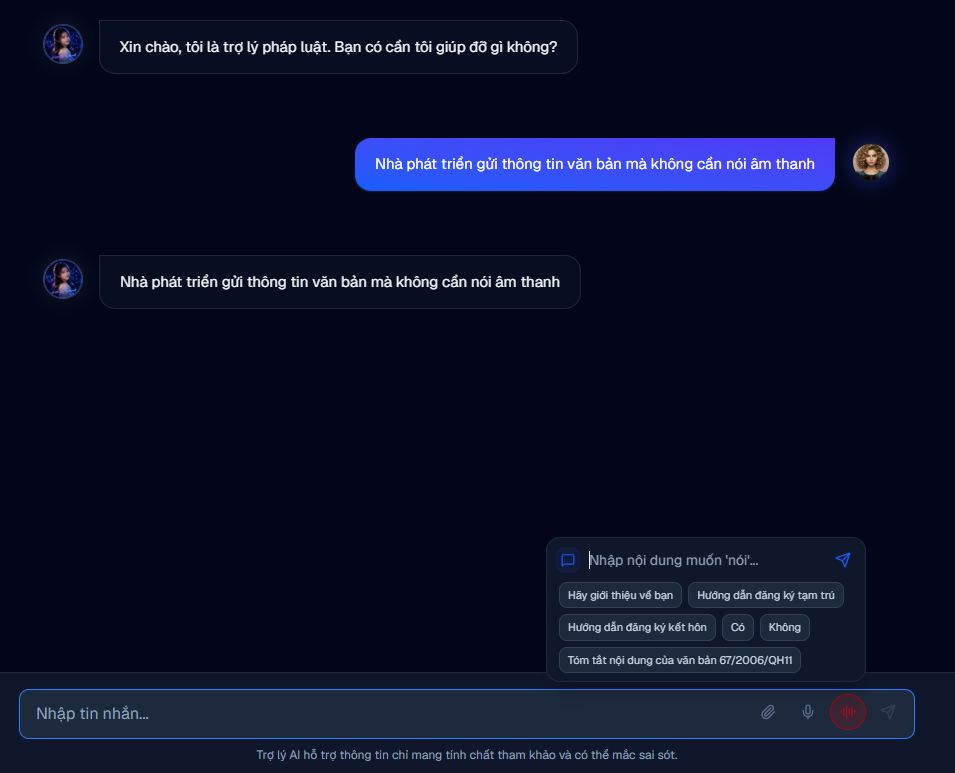
\includegraphics[height=0.7\textheight,width=0.9\textwidth,keepaspectratio]{pictures/voice-developer-send-text.png}
% \caption{Nhà phát triển gửi tin nhắn văn bản thay giọng nói để debug}
% \end{figure}

% \note{
% Trong quá trình phát triển và kiểm thử dịch vụ giọng nói, việc phát âm thanh liên tục rất bất tiện.
% Hệ thống hỗ trợ cơ chế debug cho phép nhà phát triển gửi thông tin văn bản trực tiếp thông qua Data Channel của WebRTC thay vì gửi dữ liệu âm thanh. Voice Agent nhận được văn bản sẽ lập tức xử lý suy luận thông qua mô hình ngôn ngữ và trả về kết quả dưới dạng âm thanh để nhà phát triển kiểm tra độ chính xác của phản hồi.
% }
% \end{frame}
